\documentclass[
  captions=tableheading,
  bibliography=totoc, 
  titepage=firstiscover,
]{scrartcl}

\usepackage{blindtext} %neuer input

\usepackage{longtable} % Tabellen über mehrere Seiten

\usepackage[utf8]{inputenc} %neuer input

\usepackage{scrhack}

\usepackage[aux]{rerunfilecheck} %Warnung falls nochmal kompiliert werden muss

\usepackage{fontspec} %Fonteinstellungen

\recalctypearea{}

\usepackage[main=ngerman]{babel} %deutsche Spracheinstellung

\usepackage{ragged2e} %neuer input

\usepackage{amsmath, nccmath}

\usepackage{amssymb} %viele mathe Symbole

\usepackage{mathtools} %Erweiterungen für amsmath


\DeclarePairedDelimiter{\abs}{\lvert}{\rvert}
\DeclarePairedDelimiter{\norm}{\lVert}{\rVert}

\DeclarePairedDelimiter{\bra}{\langle}{\rvert}
\DeclarePairedDelimiter{\ket}{\lvert}{\rangle}

\DeclarePairedDelimiterX{\braket}[2]{\langle}{\rangle}{
#1 \delimsize| #2
}

\NewDocumentCommand \dif {m}
{
\mathinner{\symup{d} #1}
}


\usepackage[
  math-style=ISO,
  bold-style=ISO,
  sans-style=italic,
  nabla=upright,
  partial=upright,
  warnings-off={
    mathtools-colon,
    mathtools-overbracket,
  },
]{unicode-math}

\setmathfont{Latin Modern Math}
\setmathfont{XITS Math}[range={scr, bfscr}]
\setmathfont{XITS Math}[range={cal, bfcal}, StylisticSet=1]


\usepackage[
  locale=DE,
  separate-uncertainty=true,
  per-mode=reciprocal,
  output-decimal-marker={,},
]{siunitx}

\usepackage[autostyle]{csquotes} %richtige Anführungszeichen

\usepackage{xfrac}

\usepackage{float}

\floatplacement{figure}{htbp}

\floatplacement{table}{htbp}

\usepackage[ %floats innerhalb einer section halten
  section,   %floats innerhalb er section halten
  below,     %unterhalb der Section aber auf der selben Seite ist ok
]{placeins}

\usepackage[
  labelfont=bf,
  font=small,
  width=0.9\textwidth,
]{caption}

\usepackage{subcaption} %subfigure, subtable, subref

\usepackage{graphicx}

\usepackage{grffile}

\usepackage{booktabs}

\usepackage{microtype} %Verbesserungen am Schriftbild

\usepackage[
backend=biber,
]{biblatex}

\addbibresource{../lit.bib}

\usepackage[ %Hyperlinks im Dokument
  german,
  unicode,
  pdfusetitle,
  pdfcreator={},
  pdfproducer={},
]{hyperref}

\usepackage{bookmark}

\usepackage[shortcuts]{extdash}

%\usepackage{warpcol}


\begin{document}
    \title{ATP Übungsblatt 1}
    \author{  
    Tobias Rücker\\
    \texorpdfstring{\href{mailto:tobias.ruecker@tu-dortmund.de}{tobias.ruecker@tu-dortmund.de}
    \and}{,} 
    Paul Störbrock\\
    \texorpdfstring{\href{mailto:paul.stoerbrock@tu-dortmund.de}{paul.stoerbrock@tu-dortmund.de}}{}
    }
\maketitle
\center{\Large Abgabegruppe: \textbf{Mittw. 10-12 Uhr}}
\thispagestyle{empty}

\newpage
\tableofcontents
\thispagestyle{empty}
\newpage

\setcounter{page}{1}


\section{Aufagabe 1}

\begin{figure}[H]
    \centering
    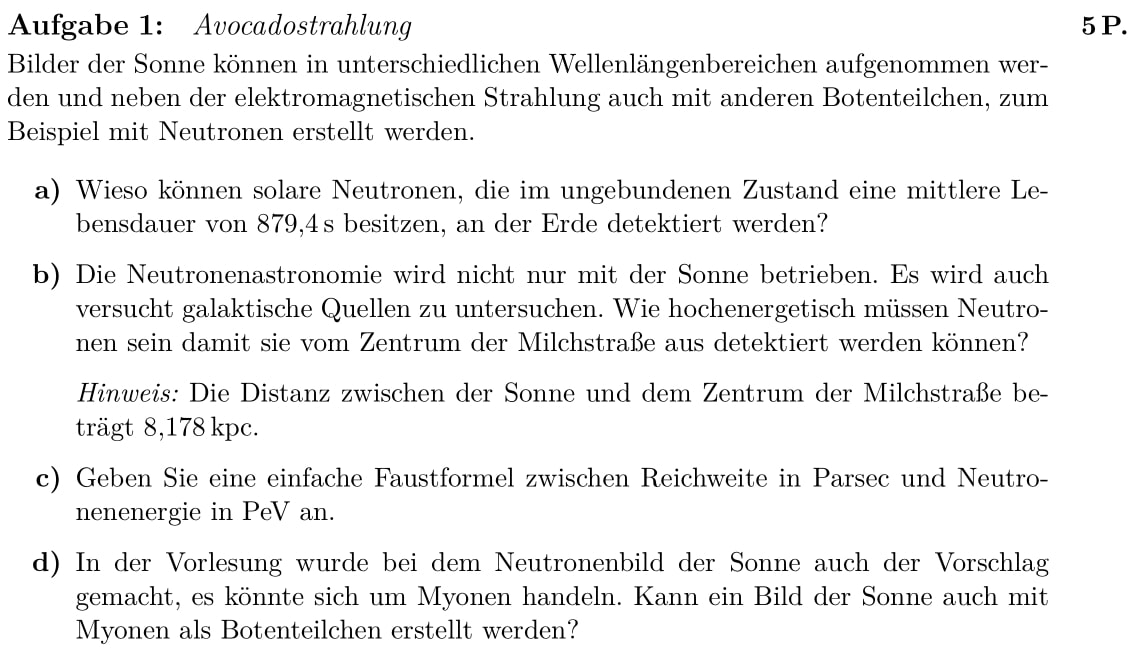
\includegraphics[width=0.75\textwidth]{images/Aufgabe_1.jpg}
    \label{fig:1}
\end{figure}

\subsection{a)}

    \flushleft{Das\;}\justifying Neutron hat eine finite Lebensdauer von ca. \SI{879.4}{\second}. Mit der Formel 
    \begin{align}
        v = \frac{d}{t} \Leftrightarrow v \cdot t = d \label{eq:1}
    \end{align}
    lässt sich die zurückgelegte Distanz bestimmen. Da das Neutron mit annähernder Lichtgeschwindigkeit propagiert ($v \~{c}$), kann man als Reisedauer des Neutrons die Lebensdauer 
    für $t$ einsetzen. Da sich das Neutron mit ungefährer Lichtgeschwindigkeit fortbewegt, muss die Distanz relativistisch, also mit der Formel
    \begin{align}
        \gamma \cdot v \cdot t = d \qquad \qquad \text{mit\;} \gamma = \frac{1}{\sqrt{1-\frac{v^2}{c^2}}} \label{eq:2}
    \end{align}
    bestimmt werden. Da $v$ hier gegen die Lichtgeschwindigkeit $c$ konvergeiert, kürtzt sich $\gamma$ weg, und es bleibt Formel \eqref{eq:1} stehen. 
    Somit ergibt sich für die maximale Distanz, die ein Neutron während dessen Lebensdauer zurücklegen kann:
    \begin{align}
        3 \cdot 10^8 \sfrac{m}{s} \cdot \SI{879.4}{\second} = \text{\input{d.tex}} \Leftrightarrow \text{\input{d_AU.tex}}
    \end{align}
    Demnach könnte ein Neutron bei annähernder Lichtgeschwindigkeit \SI{176}{\percent} der Stecke zwischen Erde und Sonne zurücklegen, was uns erlaubt Neutronen auf der Erde zu beobachten.

\subsection{b)}

    \flushleft{Die\;}\justifying relativistische Gesamtenergie $R_{ges}$ wird mit der Ruheenergie $R_0$, der Ruhemasse $m_0$ und der kinetischen Energie $E_{kin} = c^2 \cdot p^2$ bestimmt:
    \begin{align}
        E_{ges}^2 &= E_0^2 + c^2 \cdot p^2 \qquad \qquad \text{mit\;} p = m_0 \cdot v\\
        E_{ges}^2 &\stackrel{relativistisch}{=} E_0^2 + \frac{c^2 \cdot m_0^2 \cdot v^2}{1-\frac{v^2}{c^2}} \label{eq:3}
        \intertext{Wird Formel \eqref{eq:2} nach $v$ umgestellt und in \eqref{eq:3} eingesetzt, kürtzt sich das $\gamma$ raus und es folgt:
        }
        E_{ges}^2 &= d^2 t^2 \cdot c^2 m_0^2 - m_0^2 c^2
    \end{align} 


\subsection{c)}

\subsection{d)}

    \flushleft{Ein\;}\justifying Myon hat eine Halbwertszeit von \SI{1.52}{\micro\second}. Um die Erde mit relativistischer Geschwindigkeit zu erreichen, bräuchte ein Teilchen 
    \textasciitilde \SI{499}{\second}. Demnach würde das Myon auf dem Weg zerfallen und kann deswegen nicht von der Erde aus beobachtet werden. 





\section{Aufgabe 2}

\begin{figure}[H]
    \centering
    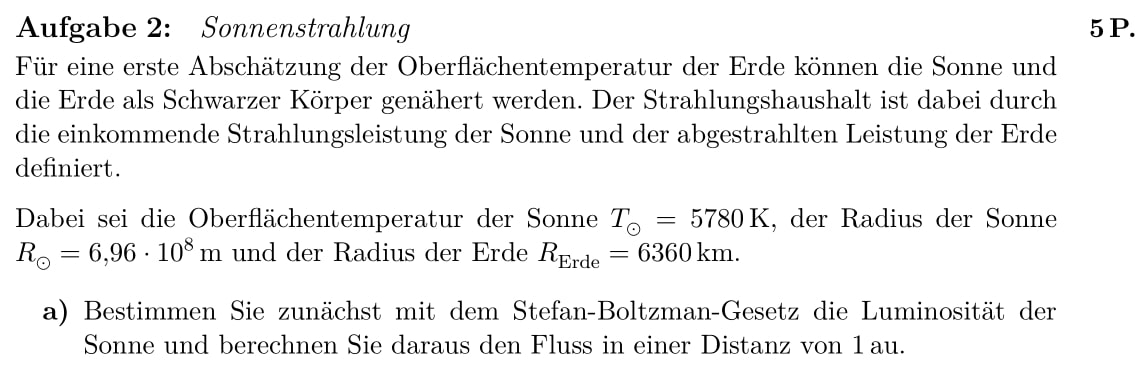
\includegraphics[width=0.75\textwidth]{images/Aufgabe_2a.jpg}
    \label{fig:2}
\end{figure}

\begin{figure}[H]
    \centering
    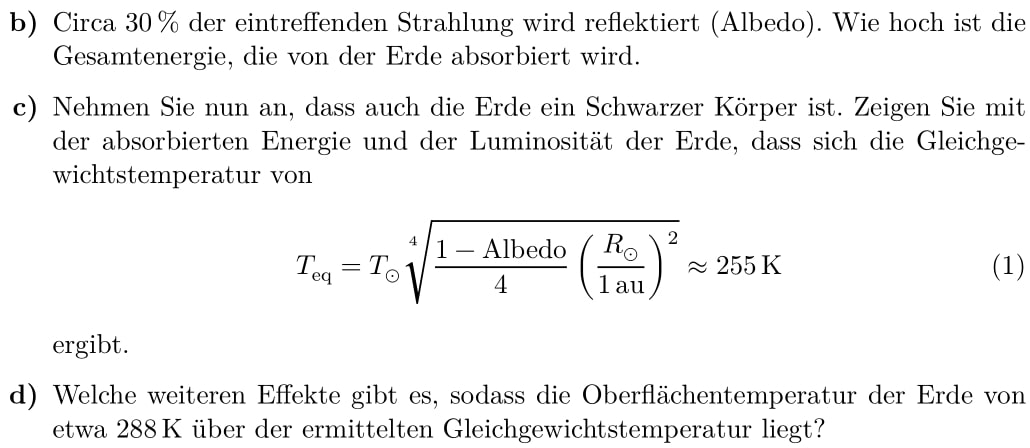
\includegraphics[width=0.75\textwidth]{images/Aufgabe_2bcd.jpg}
    \label{fig:2}
\end{figure}

\subsection{a)}

    \begin{align}
        \intertext{\flushleft{Das\;}\justifying Stefan-Boltzmann-Gesetz lautet
        $P = \sigma \cdot A \cdot T^4$, wobei P die Luminosität der Schwarzkörpers ist.
        }
        A= 4 \pi R_{Sonne}^2 
    \end{align}

        \begin{table}[H]
        \centering
        \begin{tabular}{l c}
            \toprule
                $T_{\text{Sonne}}$      & \input{T_S.tex}\\
                $R_{\text{Sonne}}$      & \input{R_S.tex}\\
                $R_{\text{Erde}}$       & \input{R_E.tex}\\
            \bottomrule
        \end{tabular}
        \caption{Messwerte}
        \label{tab:2a}
        \end{table}


    
    \begin{align}
        \intertext{\flushleft{Die\;}\justifying Luminosität der Sonne beträgt:
        }
        P_{Sonne} = \text{\input{P_S.tex}}
    \end{align}
    Die Flussdichte der Sonne in Distanz von $1$au
    \begin{align}
        f &= \frac{P_{\text{Sonne}}}{4 \pi R^2} =\frac{4 \pi R_{\text{Sonne}}^2 \sigma T^4}{4 \pi R^2}  = \frac{R_{\text{Sonne}}^2 \sigma T^4}{R^2}
        &= \SI{1368.95}{\watt\meter\tothe{-2}} 
    \end{align}

    

\subsection{b)}

Der Absoptionsfaktor für die Erdatmosphäre ist 0,7. Die Energieaufnahme beträgt dann
\begin{align}
    L &= 0,7 \cdot f_{1au} \cdot A_{\text{Erde}} = 0,7 \cdot \SI{1368.95}{\watt\meter\tothe{-2}} \pi \SI{6360e3}{\meter}
    &= \SI{173}{\peta\watt}
\end{align}



\subsection{c)}

\begin{align}
P_{eq} &= P_{ein}-P_{aus}\\
4 \sigma \pi R^2 T_{eq}^4 &= \pi R^2 f - Albedo\, \pi R^2 f\\
4 \sigma T_{eq}^4 &= (1-Albedo)f\\
4 \sigma T_{eq}^4 &= (1-Albedo) \frac{R_{\text{Sonne}}^2 \sigma T^4}{R^2}\\
T_{eq} & = T_{\text{Sonne}} \sqrt{\frac[4]{1-Albedo}{4}\left(\frac{R_{\text{Sonne}}}{R} \right)^2 }\\
T_{eq} & = T_{\text{Sonne}} \sqrt{\frac[4]{1-Albedo}{4}\left(\frac{R_{\text{Sonne}}}{1au} \right)^2 } \approx \SI{255}{\kelvin} \\
\end{align}

\subsection{d)}

\flushleft{Ein\;}\justifying Teil der Strahlung, welche von der Erde reflektiert wird, gelangt in die Atmosphäre und
regt Schwingungen bei Treibhausgasen an. Diese emittieren die Strahlung zurück auf die Erde,
wovon wiederum ein Teil absorbiert wird.
Ein anderer Teil der Erdwärme entsteht wiederum durch vulkanische Aktivitäten und ähnliches.

\section{Aufgabe 3}

\begin{figure}[H]
    \centering
    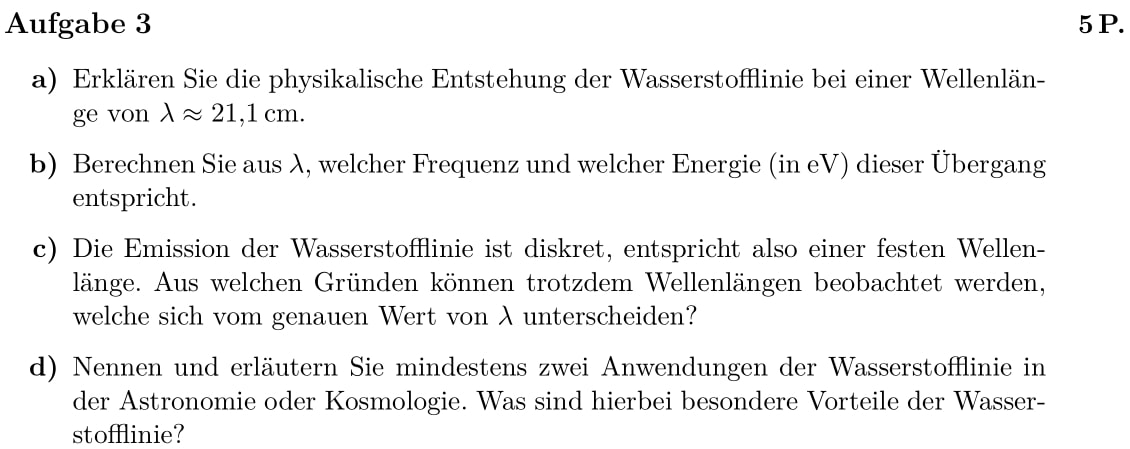
\includegraphics[width=0.75\textwidth]{images/Aufgabe_3.jpg}
    \label{fig:3}
\end{figure}

\subsection{a)}

\flushleft{Die\,}\justifying Wasserstofflinie der Wellenlänge $\lambda = \SI{21}{\centi\meter} $ ensteht durch den
Hyperfeinstrukturübergang des Wasserstoffatoms. Bei einem Wasserstoff können
die Spins entweder parallel oder entgegen gesetzt zueinander ausgerichtet sein.
Dabei ist die parallele Ausrichtung der enretisch höhere Zustand. Bei einem
Übergang von dem parallelen zum entgegengesetzten Zustand dem "Spin-Flip" wird
die H1 Linie ausgesendet.


\subsection{b)}

\flushleft{Die\,}\justifying Frequenz der H1-Wellenlänge beträgt:
\begin{align*}
    f_{H1}=\text{\input{f_H1.tex}}
\end{align*}
und die Energie zur Wellenlänge $\lambda = \SI{21}{\centi\meter} $ beträgt
\begin{align}
    E_{H1}=\text{\input{E_H1.tex}}
\end{align}


\subsection{c)}

\flushleft{Die\,}\justifying Wellenlängen der Wasserstofflinie mögen fest sein, allerdings bewegen sich
die Quellen, wodurch der Dopplereffekt auftritt. Lichtwellen vom z.B. sichbaren Spektrum deren Quellen sich vom
Beobachter entfernen werden ins rote verschoben, während Quellen, die sich auf den
Beobachter zubewegen ins blaue verschoben werden. Dadurch werden auch andere Wellenlängen  
beobachtet. 


\subsection{d)}

Die Wasserstofflinie wird in der Astrologie benutzt, um die Geschwindigkeiten 
interstellarer Gaswolken relativ zu Erde zu bestimmen. Über de auftretenden Dopplereffekt wurde
die Rotationsgeschwindigkeit der Milchstraße gemessen.


\end{document}